\documentclass{beamer}

\usepackage[sfdefault]{cabin}
\usepackage[utf8]{inputenc}
\usepackage[T1]{fontenc}
\usepackage[french]{babel}
\usepackage{xcolor}
\usepackage{caption}
\usepackage{graphicx}
%Police
%\usepackage[sfdefault]{roboto}
\usepackage[sfdefault]{FiraSans}

\definecolor{modernblue}{RGB}{70,130,180} 
\definecolor{modernvert}{RGB}{0, 80, 0} 

\usetheme{Madrid}

\usecolortheme[named=modernblue]{structure}

\setbeamertemplate{caption}{\insertcaption} % Utiliser le format de légende par défaut de Beamer

\title{UMAP : Uniform Manifold Approximation and Projection}
\author{Youness et Ivanhoé}
\date{28 octobre 2023}

\renewcommand{\thesection}{\Roman{section}}\renewcommand{\thesubsection}{\arabic{subsection} }\renewcommand{\thesubsubsection}{\alph{subsubsection} }

\newcommand{\C}{\mathbb{C}}\newcommand{\R}{\mathbb{R}}\newcommand{\Q}{\mathbb{Q}}\newcommand{\Z}{\mathbb{Z}}\newcommand{\N}{\mathbb{N}}\newcommand{\V}{\overrightarrow}\newcommand{\Cs}{\mathscr{C}}\newcommand{\Ps}{\mathscr{P}}\newcommand{\Rs}{\mathscr{R}}\newcommand{\Gs}{\mathscr{G}}\newcommand{\Ds}{\mathscr{D}}\newcommand{\happy}{\huge\smiley}\newcommand{\sad}{\huge\frownie}\newcommand{\alors}{\Large\Rightarrow}\newcommand{\equi}{\Leftrightarrow}
\newcommand{\disp}{\displaystyle}\newcommand{\Pro}{\mathbb{P}}


\newtheorem{thm}{Théorème}
\newtheorem{rmq}{Remarque}
\newtheorem{prop}{Propriété}
\newtheorem{cor}{Corollaire}
\newtheorem{lem}{Lemme}
\newtheorem{prop-def}{Propriété-définition}

\theoremstyle{definition}

\newtheorem{defi}{Définition}
\newtheorem{intro}{Initialisation}
\newtheorem{boucle}{Boucle principale}
\newtheorem{ex}{Exemple}
\newtheorem*{rap}{Rappel}
\newtheorem{cex}{Contre-exemple}
\newtheorem{exer}{Exercice} % \large {\fontfamily{ptm}\selectfont EXERCICE}
\newtheorem{nota}{Notation}
\newtheorem{ax}{Axiome}
\newtheorem{appl}{Application}
\newtheorem{csq}{Conséquence}
\def\di{\displaystyle}



\begin{document}
\begin{frame}[plain]
    \maketitle
\end{frame}


\begin{frame}
\frametitle{Introduction}

	\begin{minipage}[c]{1\linewidth}
	\begin{minipage}[t]{0.4\linewidth}\centering\begin{figure}
			\centering
			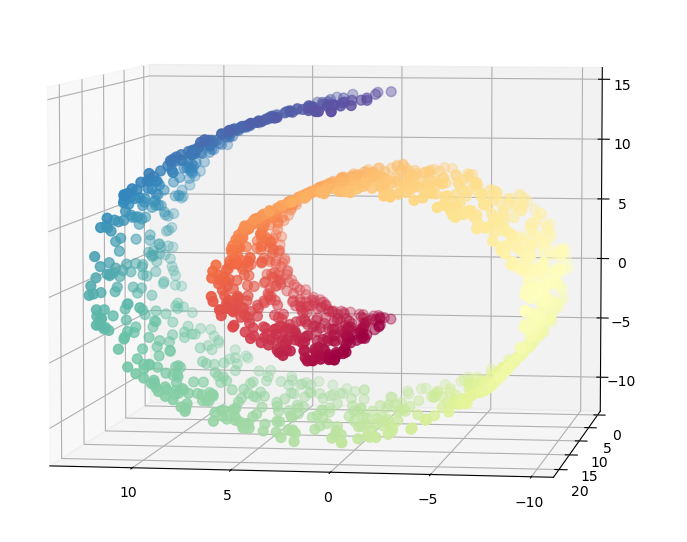
\includegraphics[scale=0.25]{swiss_roll.png}
			\caption{Représentation 3D du swiss roll dataset.}
	\end{figure}\end{minipage}\hfill 
	\begin{minipage}[t]{0.43\linewidth}\centering\begin{figure}
			\begin{center}
				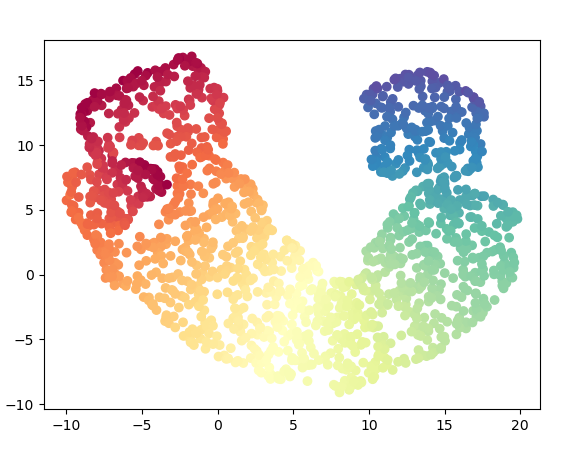
\includegraphics[scale=0.27]{umap_swiss_roll.png}			
				\caption{UMAP projection (n\_neighbors=15, min\_dist = 0.1).}
			\end{center}
			
	\end{figure}\end{minipage}
	\end{minipage}
\textcolor{modernvert}{\textbf{Problématique :}} Comment fonctionne l'algorithme UMAP et pourquoi utiliser cette méthode sur un jeu de données ?
\end{frame}

\begin{frame}
	\tableofcontents
\end{frame}

\section{Les intérêts de la méthode UMAP sur un jeu de données}
\begin{frame}
	\frametitle{Les intérêts de la méthode UMAP sur un jeu de données}
	\begin{enumerate}[$\star$]
		\item Méthode de \emph{réduction de dimension} utile pour la visualisation des données.
		\item Projection dans un espace de plus petite dimension pour des données non-linéaires donc non-séparables par un sous-espace vectoriel. 
		\item Retransmettre dans un espace de plus petite dimension la structure topologique des données initiales. 
		\item Utile pour faire du clustering et peut servir pour entraîner des modèles de machine learning. 
	\end{enumerate}
	
\end{frame}

\begin{frame}
	\begin{minipage}[c]{1\linewidth}
		\begin{minipage}[t]{0.4\linewidth}\centering\begin{figure}
				\centering
				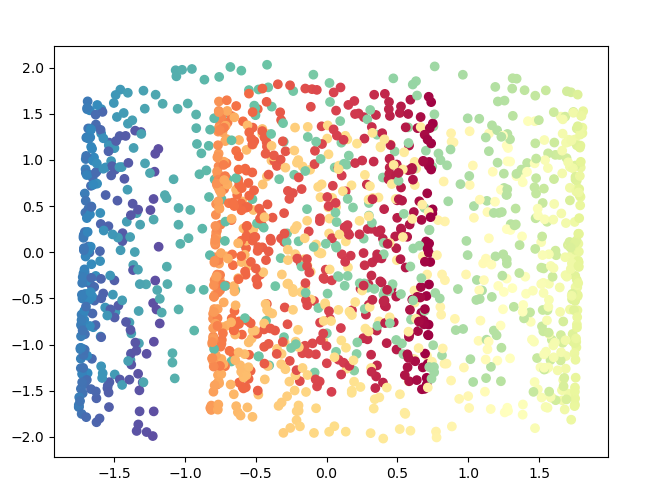
\includegraphics[scale=0.25]{acp_swiss_roll.png}
				\caption{Scatter plot de l'ACP du dataset swiss roll avec les deux premières composantes principales}
		\end{figure}\end{minipage}\hfill 
		\begin{minipage}[t]{0.43\linewidth}\centering\begin{figure}
				\begin{center}
					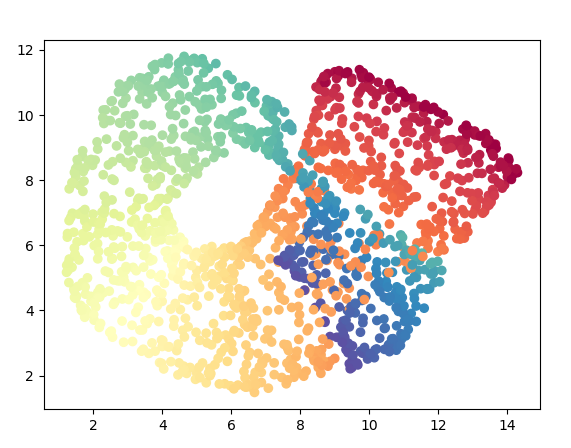
\includegraphics[scale=0.27]{umap2_swiss_roll.png}			
					\caption{UMAP projection du nuage de points dans un plan.\\ 
					(n\_neighbors=500, min\_dist = 0.5) }
				\end{center}
				
		\end{figure}\end{minipage}
	\end{minipage}
	
	
\end{frame}


\section{Présentation théorique de la méthode UMAP}
\begin{frame}
\frametitle{Présentation théorique de la méthode UMAP}
\begin{rmq}
	L'algorithme de UMAP ressemble à celui de T-SNE. Il est présenté comme plus rapide et pouvant s'adapter à une réduction de la dimension $d\geq2$. UMAP préserve aussi davantage la structure globale du jeu de donnés par rapport à T-SNE. %Il est plus stable face à la répétition du procédé car les conditions initiales ne sont pas choisies aléatoirement.
\end{rmq}
\quad \\[0.15cm]
	\textcolor{modernvert}{\textbf{Idée :}}\\ Pour un jeu de données $X\in\mathcal{M}_{n,p}(\R)$ nous cherchons à préserver les relations locales entre les individus dans un espace de dimension plus petit ($d \lll p$). Cela revient à trouver $Y\in\mathcal{M}_{n,d}(\R)$ sous certaines contraintes.\\
	
	
\end{frame}

\begin{frame}
\textcolor{modernvert}{\textbf{Les étapes importantes :}}\\[0.5cm]
\begin{enumerate}
	\item  Pour un nombre de voisins k fixé, donner pour tout couple d'individus $(x_i,x_j)$ une probabilité $p_{i,j}$ d'appartenir à un même voisinage.
	\item Initialiser la matrice $Y$ et en déduire la similarité entre les couples d'individus $(y_i,y_j)$ que l'on note $q_{i,j}$.
	\item Minimiser sur l'espace d'arrivée une fonction objectif d’entropie croisée qui mesure la dissimilarité entre les deux distributions $p$ et $q$. Ici $q$ est une fonction de $Y$.
\end{enumerate}	
	
\end{frame}

\subsection{Matrice de probabilités jointes sur l'espace de départ}
\begin{frame}
\frametitle{Matrice de probabilités jointes sur l'espace de départ}
\begin{enumerate}
	\item Fixons $k\geq 2$ le nombre de voisins à considérer. Soit $x_i,x_j$ deux individus, la similarité $p_{i|j}$ entre deux observations est définie par :$$p_{i|j} = \exp\left(-\dfrac{\max(0,\|x_i -x_j\|-\rho_i)}{\sigma_i}\right)$$

	\begin{itemize}
		\item  On définit $\rho_i = \underset{v\neq i}{\min}\|x_i-x_v\|$.
		\item L'individu $i$ est l'un des $k$ voisins de l'individu $i$ et on définit $\sigma_i$ de telle sorte que $\displaystyle \sum_{v=1}^{k}\exp\left(-\dfrac{\max(0,\|x_i -x_v\|-\rho_i)}{\sigma_i}\right) = \log_2(k)$
	\end{itemize}
	\item Symétrisation pour obtenir la probabilité d'appartenir à un même voisinage : 
	$$p_{i,j} = p_{i|j} + p_{j|i} - p_{i|j} \times p_{j|i}$$ 
\end{enumerate}


	
\end{frame}

\subsection{Similarité entre les individus de l'espace d'arrivé}
\begin{frame}
	\frametitle{Similarité entre les individus de l'espace d'arrivé}
	Fixons une distance minimale \textit{"min\_dist"}.
	\begin{enumerate}
		\item Nous aimerions définir la similarité entre deux individus $y_i,y_j$ de la manière suivante : 
		
	 $$q_{i,j} = \left\{ \begin{array}{ccc}
			1 &\text{ si } & \|y_i-y_j\|\leq \textit{min\_dist}\\
			\exp(-\|y_i-y_j\|) &\text{ si } & \|y_i-y_j\|> \textit{min\_dist}
		\end{array}\right.$$
	
		\item Pour cela on s'inspire d'une loi de Student et on pose:
		$$q_{i,j} = \left(1+ a\|y_i-y_j\|^{2b}\right)^{-1}$$ 
		L'algorithme UMAP optimise les deux paramètres $(a,b)$ pour coller au mieux à la fonction précédente qui est définie par morceaux.  
	\end{enumerate}
	
	
\end{frame}

\subsection{Fonction d'entropie croisée et minimisation}
\begin{frame}
	\frametitle{Fonction d'entropie croisée et minimisation}

	\textcolor{modernvert}{\textbf{But :}} trouver la distribution des points $y_i$ dans l'espace d'arrivée telle que les probabilités $q_{i,j}$ s'approchent le plus possible des probabilités $p_{i,j}$.
	\begin{itemize}
		\item Une fonction d’entropie croisée reliée à la divergence de Kullback-Leiber : 
		
	\end{itemize}
\begin{align*}
	CE(y_1,\cdots,y_n) =& \ CE(p,q) = \sum_{i=1}^{n}\sum_{j=1}^{n}p_{i,j}\ln\left(\dfrac{p_{i,j}}{q_{i,j}}\right) + (1-p_{i,j})\ln\left(\dfrac{(1-p_{i,j})}{(1 - q_{i,j})}\right)\\
	=&\  KL(p,q) + KL(1-p,1-q)
\end{align*}\quad\\[-0.25cm]
\begin{itemize}
		
		\item Minimiser la fonction d'entropie croisée à l'aide d'une descente de gradient stochastique :\\[-0.25cm]
		
		$$y_i : = y_i -\alpha \nabla_iCE (y_1,\cdots,y_i,\cdots,y_n)$$
		 
	\end{itemize}
	
		Pour la descente de Gradient Stochastique une seule observation est utilisée pour calculer le gradient à chaque itération et celle-ci est choisie de manière aléatoire.
	
\end{frame}


\section{Utiliser UMAP au quotidien et ses résultats}
\begin{frame}
	\frametitle{Utiliser UMAP au quotidien et ses résultats}
	\begin{itemize}
		\item Installer umap-learn et le charger.\\[0.25cm]
		
		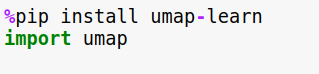
\includegraphics[scale=0.3]{1.png}
		
		\item Charger un jeu de donnés type Swiss\_Roll.\\[0.25cm]

		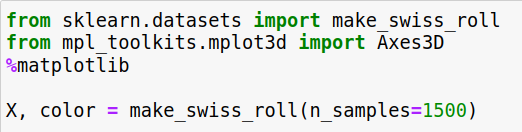
\includegraphics[scale=0.3]{2.png}
		
		\item Entraînement et projection dans le plan.\\[0.25cm]
		
		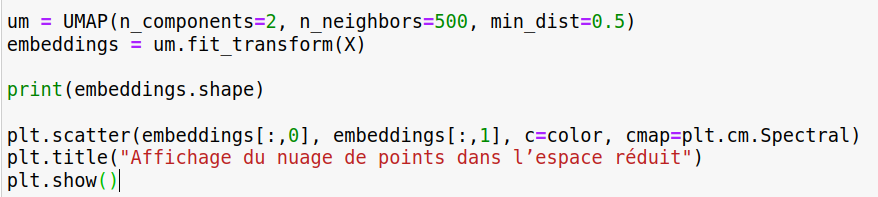
\includegraphics[scale=0.3]{3.png}
		
	\end{itemize}
	
\end{frame}

\begin{frame}
	\begin{figure}
		\centering		
		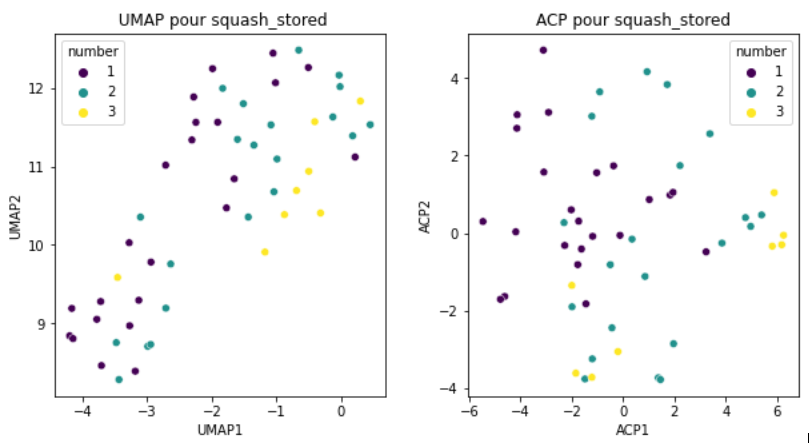
\includegraphics[scale=0.4]{squash_stored.png}
		\textit{umap.UMAP(init=X\_acp,n\_neighbors=25, min\_dist=0.02, n\_components=2)}
	\end{figure}
	
\end{frame}

\begin{frame}
	\begin{figure}
		\centering		
		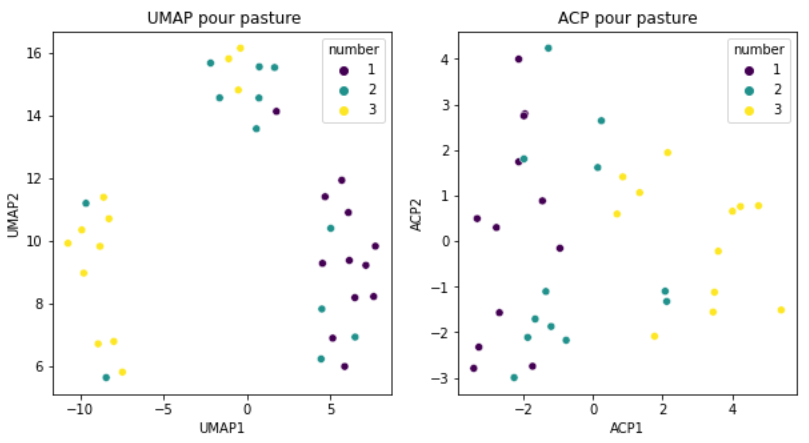
\includegraphics[scale=0.4]{pasture.png}
		\textit{umap.UMAP(init=X\_acp,n\_neighbors=5, min\_dist=1, n\_components=2)}
	\end{figure}
	
\end{frame}

\begin{frame}
	\begin{figure}
		\centering		
		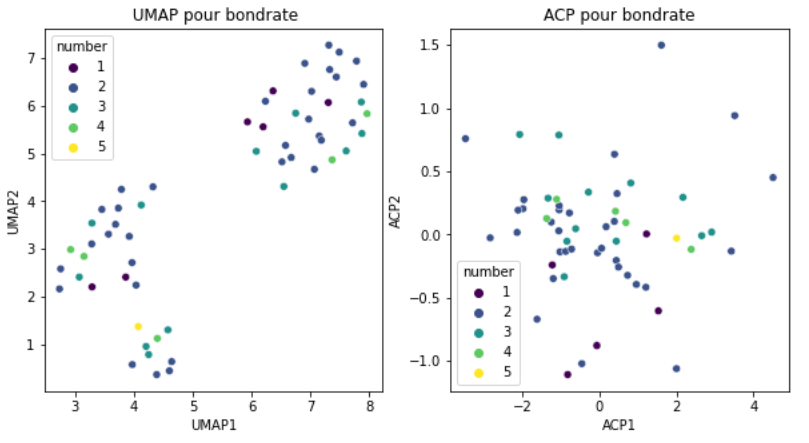
\includegraphics[scale=0.4]{bondrate.png}
		\textit{umap.UMAP(init=X\_acp,n\_neighbors=25, min\_dist=0.1, n\_components=2)}
	\end{figure}
	
\end{frame}

\begin{frame}
	\begin{figure}
		\centering		
		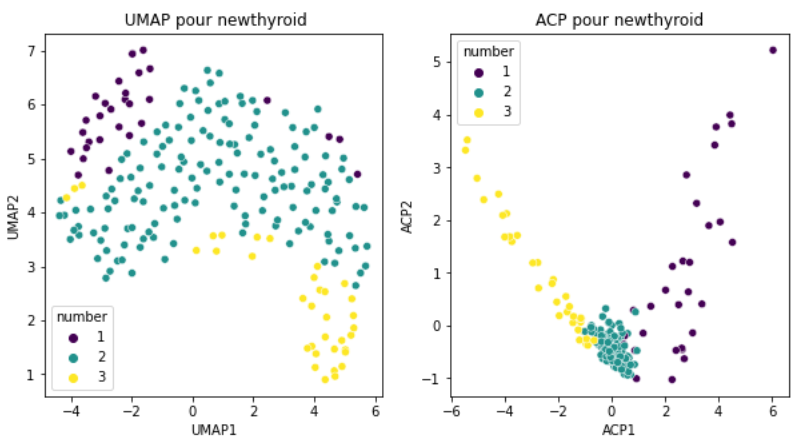
\includegraphics[scale=0.4]{thyroide.png}
		\textit{umap.UMAP(init=X\_acp,n\_neighbors=100, min\_dist=0.5, n\_components=2)}
	\end{figure}
	
\end{frame}

\section{Conclusion et faiblesses de UMAP}

\begin{frame}
	\frametitle{Faiblesses de UMAP}
	\begin{itemize}

		
		\item[$\textcolor{red}{\bullet}$] UMAP est une méthode non-paramétrique  donc il est impossible de projeter une nouvelle observation, il faut refaire l’optimisation.\\[0.5cm] 
		\item[$\textcolor{red}{\bullet}$] À l'inverse d'une méthode de réduction de dimension par projection linéaire type ACP, avec UMAP les coordonnées des observations dans l'espace d'arrivée sont moins interprétables physiquement.\\[0.5cm]  
		\item[$\textcolor{red}{\bullet}$] La recherche des bons paramètres \textbf{n\_neighborgs} et \textbf{min\_dist} n'est pas  évidente et ne permet pas toujours de rendre une vision globale des données initiales.  
	\end{itemize}
	
\end{frame}

\begin{frame}
	\frametitle{Conclusion}
	\begin{itemize}
		
		\item[$\textcolor{modernvert}{\bullet}$] Pour des datasets qui présentent une structure topologique marquée dans chaque sous groupe, les rendus de l'algorithme UMAP sont visibles et permettent bien de visualiser les clusters. \\[0.5cm] 
		
		\item[$\textcolor{modernvert}{\bullet}$] Ainsi avec UMAP sur Digits, votre modèle de machine learning type KNN ou Random Forest obtient des meilleurs scores et devient plus rapide à l'exécution. \\[0.25cm]
	\end{itemize}

	\begin{minipage}[t]{1\linewidth}
	\begin{minipage}[t]{0.3\linewidth}\centering\begin{figure}
			\centering
			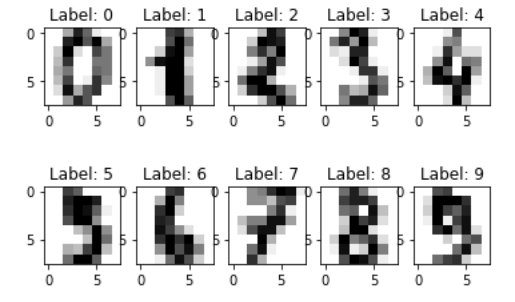
\includegraphics[scale=0.2]{digits.png}
			\caption*{Digits Dataset.}
	\end{figure}\end{minipage}\hfil 
	\begin{minipage}[t]{0.3\linewidth}\centering\begin{figure}
			\begin{center}
				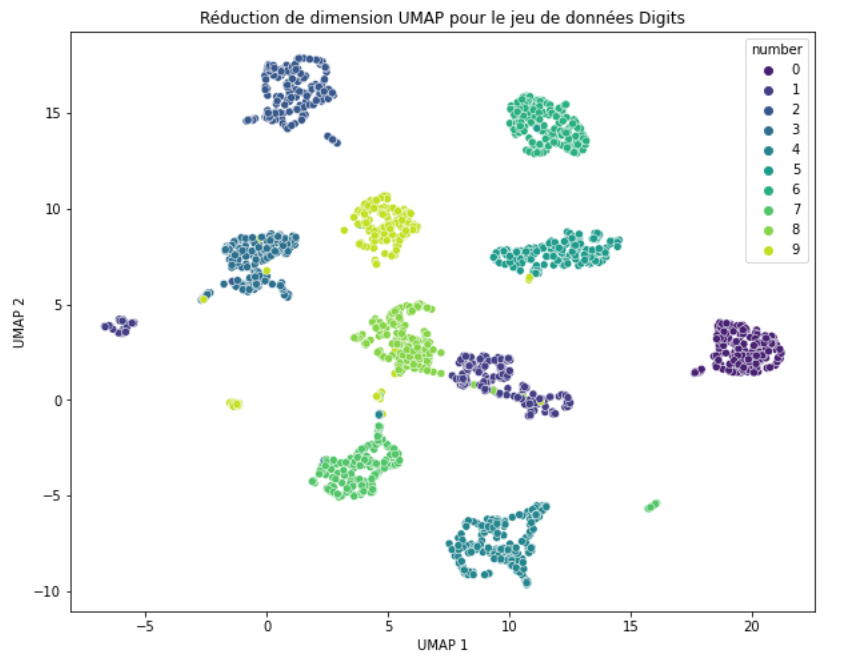
\includegraphics[scale=0.12]{umap_digits.png}			
				\caption*{UMAP projection Didgits.}
			\end{center}
			
	\end{figure}\end{minipage}\hfil \begin{minipage}[t]{0.3\linewidth}\centering\begin{figure}
\begin{center}
	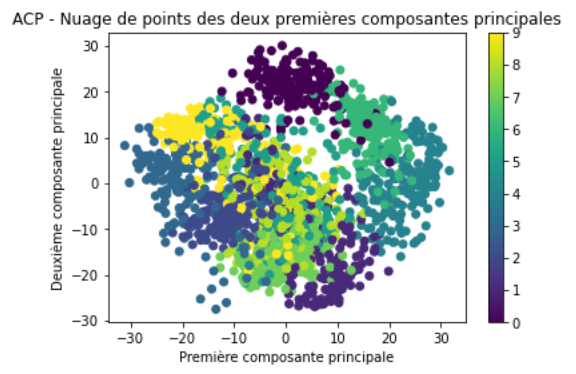
\includegraphics[scale=0.2]{acp_digits.png}			
	\caption*{ACP Didgits}
\end{center}

\end{figure}\end{minipage}
\end{minipage}


	
\end{frame}

\end{document}








